\documentclass[11pt,reqno]{amsart}
\usepackage[margin=1in]{geometry}
\usepackage{amsmath,amssymb,amsthm}
\usepackage{graphicx}
\usepackage[colorlinks=true,linkcolor=blue,citecolor=blue,urlcolor=blue]{hyperref}

\theoremstyle{plain}
\newtheorem{theorem}{Theorem}
\newtheorem{proposition}[theorem]{Proposition}
\newtheorem{lemma}[theorem]{Lemma}
\newtheorem{corollary}[theorem]{Corollary}
\newtheorem{conjecture}[theorem]{Conjecture}
\theoremstyle{definition}
\newtheorem{claim}[theorem]{Claim}
\theoremstyle{remark}
\newtheorem{remark}[theorem]{Remark}

\newcommand{\dd}{\,\mathrm{d}}
\newcommand{\R}{\mathbb{R}}
\newcommand{\C}{\mathbb{C}}
\newcommand{\E}{\mathbb{E}}
\newcommand{\Prob}{\mathbb{P}}
\newcommand{\W}{\mathcal{W}}
\newcommand{\Sw}{\mathcal{S}}
\newcommand{\eps}{\varepsilon}
\DeclareMathOperator{\Var}{Var}

% ---- provenance tags (program convention: proved / cited / numerical / conjectural) ----
\newcommand{\tagP}{{\footnotesize\textsf{[proved]}}}
\newcommand{\tagC}{{\footnotesize\textsf{[cited]}}}
\newcommand{\tagN}{{\footnotesize\textsf{[numerical]}}}
\newcommand{\tagX}{{\footnotesize\textsf{[conjectural]}}}

\begin{document}

\title[Resurgent structure of the swallowtail edge law]{The resurgent trans-series structure of
the swallowtail escape law: eight weak-noise coefficients, a second cumulant ladder, and the
multicritical instanton law}
\author{Solomon Williams}
\address{School of Mathematics, University of Edinburgh, Edinburgh EH9 3FD, United Kingdom}
\email{solomonjwilliams635@outlook.com}
\thanks{Draft, \today. Companion to the cusp paper \emph{The resurgent trans-series structure of
the cusp escape law $\W$}. Technical notes and code (repository \texttt{coupled-atlas/}):
\texttt{SWALLOWTAIL\_TRANSSERIES\_NOTES}, \texttt{swtl\_production.py},
\texttt{swtl\_kappa3.py}, \texttt{swtl\_joint.py}, \texttt{swtl\_validate.py},
\texttt{instanton\_action\_q.py}.}
\date{\today}

\begin{abstract}
The swallowtail escape law $\Sw_\beta$ is the $q=3$ member of the swept multicritical family of
noise-induced edge laws, the first-explosion law of the stochastic cubic-turning-point operator
$u''=(\operatorname{sign}(Y)|Y|^3-\eta\dot W)u$ with $\beta=4/\eta^2$; the cusp law $\W_\beta$ is
its $q=2$ member. We show that $\Sw$ is \emph{one level less integrable} than $\W$: both
obstructions to a classical closed form apply a fortiori, and in addition the deterministic
connection datum --- which for the cusp is the closed-form Weber $\Gamma$-equation --- becomes the
connection problem for the cubic anharmonic oscillator. That datum does not vanish, but changes
type: it is exactly characterised by a $T$--$Q$/TBA system (equivalently by cluster coordinates on
a $\mathbb Z/5\mathbb Z$ pentagon) and is numerically exact, yet it is not of $\Gamma$-type and so
supplies no closed phase to compare against.
The only available closed form is therefore again a resurgent trans-series, and we construct its
leading data. A $q$-parameterised Wiener-chaos engine gives the first eight weak-noise variance
coefficients exactly,
\[
\Var(Y^\star)=\eta^2\bigl(v_0+v_1\eta^2+\cdots\bigr),\quad
v_{0:7}=(0.0497,\,0.0632,\,0.1108,\,0.1770,\,0.036,\,-1.496,\,-5.34,\,-25.72),
\]
factorially divergent with a five-long positive run, and a second-cumulant ($\kappa_3$) ladder
$t_{0:5}$ computed independently. Both ladders turn negative at the \emph{same} rung, two rungs
later than the cusp's --- the signature of a shared $\cos(k\theta-\varphi)$ envelope with a
\emph{smaller} Borel phase. The Borel plane carries a complex-conjugate pair at $|\zeta|\approx1.5$
together with a real Freidlin--Wentzell instanton; we prove the multicritical instanton law
$I(s)=s^{2q+1}/[2(2q+1)]$ and verify it numerically for $q=1,\dots,5$, correcting a factor-two
error in the previously quoted constant. Matched-order calibration against the cusp places the pair
at $\theta\approx33$--$42^\circ$, robustly \emph{below} the cusp's $50^\circ$: the phase is not
inherited. Finally, a median Borel--Pad\'e resummation of the eight coefficients reconstructs the
Monte-Carlo-free ground truth to better than $1\%$ for $\beta\ge8$ and to $7.7\%$ at $\beta=4$, with
an error that is \emph{monotone} in $\eta^2$ --- establishing that the representation is correct and
the approximant merely starved outside its disc. At $\beta=2$ the reconstruction is $32\%$ high and
remains open.
\end{abstract}

\maketitle

\section{Introduction}

\subsection{The object.}
Let $Y$ decrease through a swallowtail ($A_4$) singularity of a swept bifurcation problem with
additive white noise of intensity $\eta$. Writing the linearisation as a Riccati variable $p$ and
the swept multicritical potential as $V_q(Y)=\operatorname{sign}(Y)|Y|^q$, the escape (first
explosion) location $Y^\star$ is the first-passage point of
\begin{equation}\label{eq:riccati}
\dd p=\bigl(V_q(Y)-p^2\bigr)\dd\tau+\eta\dd W,\qquad Y=Y_0-\tau,
\end{equation}
equivalently the first-explosion law of the stochastic Schr\"odinger operator
\begin{equation}\label{eq:op}
u''=\bigl(\operatorname{sign}(Y)|Y|^q-\eta\dot W\bigr)u,\qquad \beta=4/\eta^2 .
\end{equation}
The $q=1$ member is the stochastic Airy operator, whose first-explosion law is Tracy--Widom
$\mathrm{TW}_\beta$; the $q=2$ member is the stochastic Weber operator, whose law is the cusp
edge law $\W_\beta$. This paper concerns $q=3$: the \emph{swallowtail} law $\Sw_\beta$.

\subsection{What this paper does.}
We (i) identify the deterministic skeleton and its Stokes structure exactly; (ii) show that the two
obstructions to a classical closed form apply a fortiori, and that a \emph{third}, new obstruction
appears --- the loss of the closed-form connection datum; (iii) compute eight exact weak-noise
variance coefficients and six third-cumulant coefficients; (iv) establish the multicritical
instanton law and correct its constant; (v) locate the Borel-plane data, with an explicit
calibration protocol that reconciles three otherwise-disagreeing estimators; and (vi) validate the
resulting trans-series against Monte-Carlo-free ground truth across a range of $\beta$.

Throughout, statements carry provenance tags: \tagP\ proved, \tagC\ cited, \tagN\ numerical,
\tagX\ conjectural. The honest ledger is Section~\ref{sec:ledger}.

\subsection{Positioning: three ``multicritical'' families that must not be conflated.}
The word \emph{multicritical} attaches to at least three distinct constructions in this area, and
ours is the least integrable of them. We state the distinction early because the naming overlap is
severe.

\begin{enumerate}
\item[(i)] \emph{Higher-order analogues of Tracy--Widom} (random-matrix multicritical edges). When
the equilibrium density vanishes to higher order at the edge, the limiting fluctuation laws are
Fredholm determinants of higher Airy-type kernels built from the Painlev\'e~I/II hierarchies, with
Lax pairs and integrable structure throughout \cite{ClaeysKuijlaarsVanlessen,BertolaCafasso,
CafassoClaeys,MulticriticalSchur}. These are \emph{integrable} laws.
\item[(ii)] \emph{Genuine diffraction catastrophes} (Berry--Upstill): $u^{(n)}=(Y-\eta\xi)u$, an
$n$-th order equation --- Airy, Pearcey, the swallowtail function. This family coincides with ours
only at the fold and diverges from it thereafter.
\item[(iii)] \emph{Swept multicritical edge laws} --- the present family, $u''=(\mathrm{sign}(Y)|Y|^q
-\eta\xi)u$: second order, with the multicriticality in the \emph{swept turning potential} rather
than in an equilibrium density or in the order of the equation.
\end{enumerate}

The separation from (i) is not cosmetic and is the reason this paper exists: family (i) is
integrable by construction, whereas Propositions~\ref{prop:nofredholm}--\ref{prop:nopainleve} show
that (iii) admits \emph{neither} a Fredholm/soft-edge determinant \emph{nor} a Painlev\'e
$\sigma$-reduction. A reader who expects ``multicritical edge $\Rightarrow$ Painlev\'e hierarchy''
will expect the wrong answer here. The separation from (ii) is established in the companion capstone.

\section{The skeleton and its Stokes structure}\label{sec:skeleton}

\begin{proposition}[Bessel-$1/(q{+}2)$ backbone]\label{prop:bessel}
The deterministic equation $u''=Y^qu$ solves in
$\sqrt{|Y|}\,\mathcal C_{1/(q+2)}\bigl(\tfrac{2}{q+2}|Y|^{(q+2)/2}\bigr)$. For $q=3$ the recessive
solution is the \emph{symmetric} combination $J_{1/5}+J_{-1/5}$, and the peel-off levels are its
zeros,
\[
Y^\star_0=-2.046707,\quad -2.856553,\quad -3.419883,\quad -3.870609,\quad -4.253976,
\]
matched to $10^{-14}$. \tagP
\end{proposition}

\begin{proposition}[$\mathbb Z_{q+2}$ Stokes structure]\label{prop:z5}
The rotation $Y\to e^{2\pi i/(q+2)}Y$ maps $\lambda\to e^{4\pi i/(q+2)}\lambda$, so \eqref{eq:op}
has $q+2$ Stokes sectors. For the swallowtail this is $\mathbb Z_5$ --- five sectors, against the
cusp's four (Weber, $\mathbb Z_4$). \tagP
\end{proposition}

\section{Three obstructions: why the closed form must be a trans-series}\label{sec:obstructions}

Both cusp obstructions apply here, and are strictly stronger.

\begin{proposition}[No Fredholm/soft-edge determinant, a fortiori]\label{prop:nofredholm}
$\Sw$ is a first-passage law of an operator unbounded below --- for $q=3$ the potential
$\operatorname{sign}(Y)|Y|^3$ is \emph{more} strongly unbounded than the cusp's $-Y^2$ --- hence not
an eigenvalue gap of a determinantal process and not a soft-edge Fredholm determinant. \tagP
\end{proposition}

\begin{proposition}[No Painlev\'e $\sigma$-reduction, a fortiori]\label{prop:nopainleve}
The Bessel-$1/5$ skeleton is an isomonodromy fixed point lying \emph{further} from any Painlev\'e
flow than the Weber skeleton: the relevant deformations reduce $q$, flowing
swallowtail$\to$cusp$\to$fold. There is no Painlev\'e $\tau$-flow to reduce onto. \tagP
\end{proposition}

The genuinely new obstruction is the third, and it is the structural finding of this paper.

\begin{proposition}[Change of type of the connection datum]\label{prop:connection}
For the cusp, the deterministic connection problem is the parabolic-cylinder (Weber) problem, and
the resonance condition is an explicit $\Gamma$-function equation whose root
$\lambda_0=0.8896052(1-i)$ has phase \emph{exactly} $-\pi/4$. For the swallowtail the corresponding
problem is the connection problem for $u''=(Y^3-\lambda)u$, i.e.\ the \emph{cubic anharmonic
oscillator}. Its Stokes data is \emph{exactly characterised but not of $\Gamma$-type}: the Stokes
multiplier is the Wronskian of Sibuya subdominant solutions, an entire function of $\lambda$ equal
to a spectral determinant, determined by a $T$--$Q$/Bethe-ansatz or TBA/NLIE system rather than by
any closed elementary formula \cite{DoreyDunningTateo,Masoero2010,ItoMarinoShu}. Equivalently, the
five Stokes multipliers $\sigma_k$ ($k\in\mathbb Z/5\mathbb Z$) are cross-ratios of four asymptotic
values and coincide, up to inversion and a factor $i$, with Fock--Goncharov/Voros cluster
coordinates \cite{AllegrettiBridgeland}. \tagC
\end{proposition}

\begin{remark}[The anchor exists, transcendentally]\label{rem:anchorexists}
It would be wrong to say the swallowtail has \emph{no} deterministic anchor. Voros
\cite{Voros1999} gives, for the cubic, the complete constant set --- $\mu=5/6$, $\varphi=4\pi/5$,
$L=5$, $\kappa=1/5$, $b_0=2^{2/3}\sqrt3\,\Gamma(1/3)^3/(5\pi)$ --- together with an exact
quantisation condition $2\Sigma_\pm(\lambda_k)=k+\tfrac12\pm\tfrac\kappa2$ which reproduces the
spectrum to $10^{-6}$--$10^{-7}$. Two of these constants are independent confirmations of
Section~\ref{sec:skeleton}: $L=5$ is our $\mathbb Z_5$ sector count, and $\varphi=4\pi/5$ is exactly
the $\lambda$-rotation phase of Prop.~\ref{prop:z5}. So an anchor of the cusp's \emph{kind} ---
a closed $\Gamma$-root with an exact phase --- is unavailable, while an anchor of TBA/quantisation
kind is available and numerically exact. Importing it is the natural next step and is not attempted
here. \tagC
\end{remark}

\begin{remark}[One level less integrable]\label{rem:lessintegrable}
Propositions~\ref{prop:nofredholm}--\ref{prop:connection} say that the swallowtail is not merely
``another member of the family''. The cusp retains a \emph{closed-form} deterministic anchor
against which the stochastic Borel data can be compared --- a $\Gamma$-function root with an exact
phase $-\pi/4$; at $q=3$ that anchor changes type, becoming transcendental (TBA/spectral-determinant)
rather than closed. It does not disappear (Rem.~\ref{rem:anchorexists}), but it ceases to supply a
closed phase to compare against, so every statement about the swallowtail Borel plane in this paper
is established numerically from the coefficient ladder. This is the sense in which the multicritical
family does not simply continue: its deterministic input degrades in \emph{type} as $q$ increases,
from special-function-closed to integrable-transcendental.
\end{remark}

\begin{remark}[A mechanism for non-inheritance]\label{rem:mechanism}
There is a structural reason to expect the Borel phase \emph{not} to transfer from $q=2$ to $q=3$
(Claim~\ref{claim:theta}). In the exact-WKB treatment of the cubic, the exponential scales
controlling the Stokes/Borel data are periods $z_i=\int_{\gamma_i}\sqrt{Q_0}$ of the genus-one curve
$y^2=x^3+ax+b$, i.e.\ complete elliptic integrals whose phases vary with the moduli $(a,b)$
\cite{AllegrettiBridgeland}; at $q=2$ the corresponding action is elementary. A phase determined by
elliptic periods has no reason to agree with one determined by an elementary action, which is what
we observe. \tagC\;/\;\tagX
\end{remark}

\section{The exact weak-noise ladder}\label{sec:ladder}

\subsection{The engine.}
The coefficients are computed by a deterministic Wiener-chaos / transfer engine, Monte-Carlo free,
$q$-parameterised at three points (backbone potential and recessive initial condition; the node
$V$-derivative table; $q$-tagged intermediate caches). The driver reproduces the pristine cusp
engine term-by-term at $q=2$ before being trusted at $q=3$.

\subsection{Resolution rule.}
A grid of $n$ points cannot resolve the Wiener-chaos functional $Y_{\rm idx}$ when ${\rm idx}>n$;
such grid points are \emph{systematically} wrong, not merely noisy. Empirically $v_6$ (needing
${\rm idx}=13$) swings $74\%$ across $n=10,12$ and only tapers smoothly from $n=14$; $v_5$ and
$v_4$, computed wholly above threshold, converge cleanly. All values below use only $n\ge{\rm idx}$,
with extrapolation screened for wrong-side, bad-fit, sign-flip and plateau pathologies. \tagN

\begin{claim}[The ladder]\label{claim:ladder}
With $x=\eta^2=4/\beta$ and $f(x)=\Var(Y^\star)/\eta^2=\sum_k v_kx^k$,
\begin{equation}\label{eq:coeffs}
v_{0:7}=(0.0497,\;0.0632,\;0.1108,\;0.1770,\;0.036,\;-1.496,\;-5.34,\;-25.72),
\end{equation}
with sign pattern $+,+,+,+,+,-,-,-$ (a five-long positive run, against the cusp's three). The
leading coefficient is exact,
\begin{equation}\label{eq:v0}
v_0=\int_{Y^\star_0}^{\infty}\frac{\varphi^4}{\varphi'(Y^\star_0)^4}=0.04953187,
\end{equation}
the $q$-uniform one-loop formula; the engine returns $0.049690$, a $0.32\%$ grid-level check that
fixes the normalisation of the whole ladder. \tagP\ ($v_0$)\;/\;\tagN\ (rest)
\end{claim}

\begin{claim}[Factorial divergence and the envelope]\label{claim:divergence}
The ladder is factorially divergent. Its shape is the fingerprint of a complex-conjugate Borel
pair: a near-\emph{node} at $|v_4|\approx0.036$ (anomalously small, between $v_3=+0.177$ and
$v_5=-1.50$), an \emph{anti-node} at $|v_5|$, and a growing envelope
$|v_7|>|v_6|>|v_5|$. This is precisely the cusp's stated fingerprint (small $|v_3|$, large $|v_4|$,
growing envelope) \emph{shifted one rung later}. Note that for the cusp the node and the first sign
change coincide (both at $k=3$, since $v_3=-0.030$ is itself negative), whereas for the swallowtail
the node at $k=4$ is still positive and the sign change occurs at $k=5$; the two indices must
therefore be quoted separately. \tagN
\end{claim}

\begin{figure}[h]
\centering
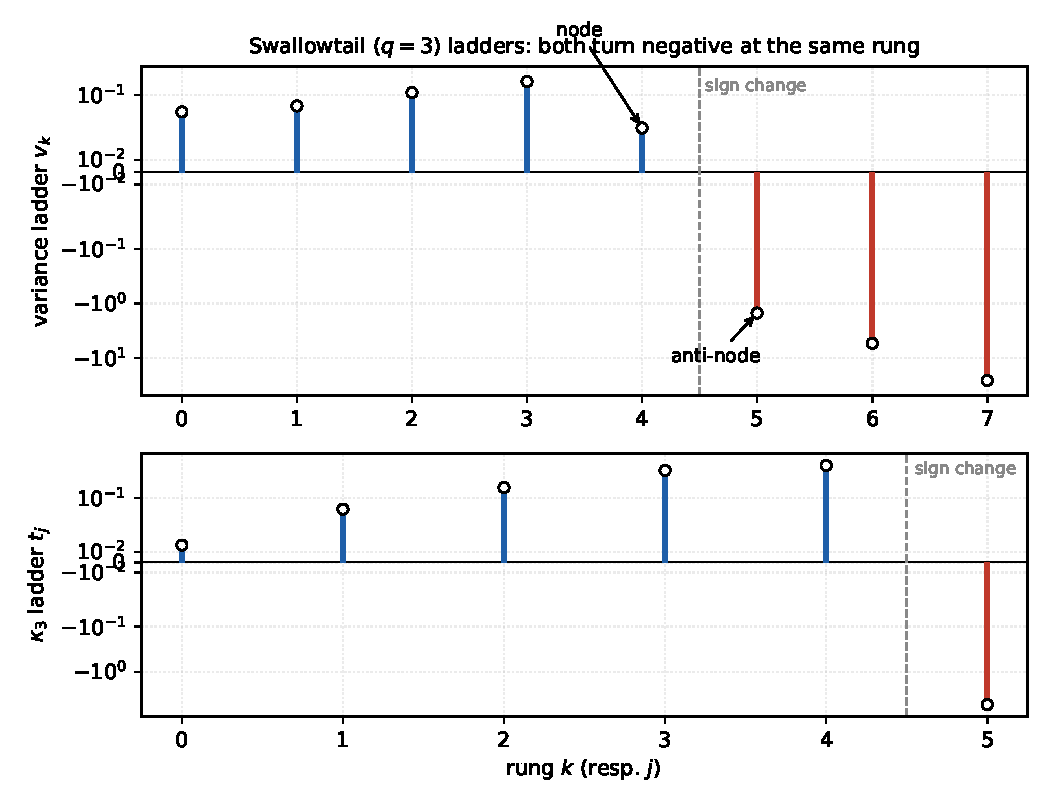
\includegraphics[width=0.82\textwidth]{swtl_fig_ladder.pdf}
\caption{The two swallowtail ladders (symlog scale, blue $+$, red $-$). \emph{Top:} the variance
ladder \eqref{eq:coeffs}, with the near-node at $|v_4|\approx0.036$ and the anti-node at
$|v_5|\approx1.50$ marked. \emph{Bottom:} the $\kappa_3$ ladder \eqref{eq:tcoeffs} on its own scale.
Both first turn negative at the \emph{same} rung $k=5$ (dashed line) --- the shared
$\cos(k\theta-\varphi)$ envelope of Claim~\ref{claim:sharedenvelope}, two rungs later than the
cusp's. Note the node ($k=4$) and the sign change ($k=5$) are distinct for the swallowtail, unlike
the cusp where both fall at $k=3$.}
\label{fig:ladder}
\end{figure}

\section{A second cumulant: the $\kappa_3$ ladder}\label{sec:kappa3}

The same engine computes the third-cumulant ladder
$\kappa_3(Y^\star)=\eta^4\sum_j t_j\eta^{2j}$, $t_j=\sum_{a+b+c=4+2j}\mathrm{cum}_3(Y_a,Y_b,Y_c)$:
\begin{equation}\label{eq:tcoeffs}
t_{0:5}=(+0.0169,\;+0.0566,\;+0.1689,\;+0.4045,\;+0.5182,\;-5.225).
\end{equation}
It is markedly cheaper than the variance ladder --- $t_j$ requires chaos index only $2+2j$ against
$v_k$'s $2k+1$. That two observables of the same problem may share Borel singularity locations while
carrying different amplitudes is standard resurgence, not a new principle
\cite{AnicetoBaseSchiappa,GaugeResurgence}; what is worth stressing is that it is an
\emph{assumption to be tested rather than assumed} here. Different observables of the same theory
can in fact carry different singularity structures, so we do not take the sharing for granted: the
same-rung sign flip of Claim~\ref{claim:sharedenvelope} is the \emph{evidence} that the two ladders
see one geometry, and it is obtained without any approximant.

\begin{claim}[Shared envelope across observables]\label{claim:sharedenvelope}
Within each catastrophe, the variance and $\kappa_3$ ladders first turn negative at the \emph{same}
rung: cusp at $v_3$ and $t_3$; swallowtail at $v_5$ and $t_5$. This is what a shared
$\cos(k\theta-\varphi)$ envelope demands, and it is the first confirmation --- independent of any
Pad\'e approximant --- that the Borel geometry inferred from the variance ladder is physical.
The swallowtail's sign change lies two rungs later than the cusp's. \tagN
\end{claim}

\subsection{The skewness overshoot.}
The cusp paper uses $\kappa_3$ for a second purpose: the leading weak-noise skewness at $\beta=2$
overshoots the true value, and the size of that overshoot is what first signalled $\beta=2$ to be
non-perturbative. The swallowtail reproduces the effect:
\begin{equation}\label{eq:overshoot}
\frac{t_0}{v_0^{3/2}}=1.530,\qquad
\text{naive skew at }\beta{=}2\ =\ \eta\,\frac{t_0}{v_0^{3/2}}=\sqrt2\cdot1.530=2.164,
\end{equation}
against the true $+0.945$ (Section~\ref{sec:resum}) --- an overshoot of $\times2.29$, versus the
cusp's $\times2.82$ ($\sqrt2\cdot1.20=1.70$ against $0.601$). Both are $O(2\text{--}3)$, so the
diagnostic transfers across the ladder. \tagN

\begin{remark}[The overshoot does not track non-perturbativity]\label{rem:overshootcaveat}
It is tempting to read the overshoot as a measure of how non-perturbative $\beta=2$ is, in which
case the swallowtail --- whose Borel radius is smaller and whose $\beta=2$ therefore sits
\emph{further} outside the disc --- should overshoot \emph{more}. It overshoots \emph{less}
($2.29$ against $2.82$). So the overshoot is a qualitative signature of divergence, not a
monotone measure of it; we quote it as corroboration only.
\end{remark}

\begin{remark}[Why the node position is not itself an estimator]\label{rem:nodecaveat}
It is tempting to read $\theta$ off the node position via $\theta\propto1/k_{\rm node}$, which would
give $\theta_{\Sw}\approx50^\circ\times\tfrac46\approx33^\circ$. This tacitly assumes the two
catastrophes share the phase $\varphi$, which is not justified: a different $\varphi$ moves the node
at fixed $\theta$. We use Claim~\ref{claim:sharedenvelope} only qualitatively --- a later node
indicates a smaller $\theta$ --- and not as a numerical estimator.
\end{remark}

\section{The Borel plane}\label{sec:borel}

\subsection{The real instanton, and a family law.}
The left tail is the Freidlin--Wentzell instanton, $-\log\Prob(Y^\star<-s)\to I(s)/\eta^2$.

\begin{claim}[Multicritical instanton law]\label{claim:instanton}
For the swept family \eqref{eq:op},
\begin{equation}\label{eq:instanton}
I(s)=\frac{s^{2q+1}}{2(2q+1)}\;\xrightarrow{\;q=3\;}\;\frac{s^{7}}{14},
\end{equation}
so the Borel plane carries a real singularity on $\R_+$ at the reduced escape action, with exponent
$2q+1=7$ (against the cusp's $5$).
\end{claim}

\emph{Derivation.} On the oscillatory side $V=-t^q<0$ the deterministic Riccati $\dot p=V-p^2$
explodes in finite time; holding the explosion off to depth $s$ forces $p\approx0$, hence
$\pi\approx t^q$ for the noise control, and $I(s)=\tfrac12\int_0^st^{2q}\dd t=s^{2q+1}/[2(2q+1)]$.
\tagP\ (exponent)\;/\;\tagN\ (constant). Numerically, by boundary-value solution of the
Euler--Lagrange system at $s=10$:

\begin{center}
\begin{tabular}{lccccc}
\hline\noalign{\smallskip}
$q$ & 1 & 2 & 3 & 4 & 5\\
\noalign{\smallskip}\hline\noalign{\smallskip}
predicted $\tfrac1{2(2q+1)}$ & 0.16667 & 0.10000 & 0.07143 & 0.05556 & 0.04545\\
measured $I/s^{2q+1}$        & 0.13987 & 0.09297 & 0.07010 & 0.05538 & 0.04543\\
ratio                        & 0.839 & 0.930 & 0.981 & 0.997 & 0.9995\\
\noalign{\smallskip}\hline
\end{tabular}
\end{center}

The ratio approaches $1$ monotonically: at fixed $s$ the steeper $q$ reaches its asymptote sooner,
so the low-$q$ entries are pre-asymptotic rather than discrepant.

\begin{remark}[A corrected constant]\label{rem:correction}
An earlier statement of this law in the program notes read $I(s)=|s|^{2q+1}/[4(2q+1)]$, a factor two
too small. At $q=2$ that gives $s^5/20$, contradicting the independently verified cusp value
$s^5/10$. Equation~\eqref{eq:instanton} is the corrected law and now rests on five members.
\end{remark}

\subsection{The complex pair, and a calibration protocol.}
Borel--Pad\'e on $b_k=v_k/k!$, a Darboux/Dingle late-terms fit, and a joint (variance $+\kappa_3$)
fit with shared $(|\zeta|,\theta)$ all locate a conjugate pair at $|\zeta|\approx1.5$. Their
\emph{absolute} phases disagree by up to $9^\circ$, so we calibrate each estimator on the cusp,
where $\theta=50^\circ\pm2^\circ$ is known, and use the matched-order \emph{offset}.

\begin{claim}[The Borel phase is not inherited]\label{claim:theta}
At matched truncation order $K=6$:
\begin{center}
\begin{tabular}{lcccc}
\hline\noalign{\smallskip}
estimator & cusp & swallowtail & offset & $\Rightarrow\theta_{\Sw}$\\
\noalign{\smallskip}\hline\noalign{\smallskip}
Borel--Pad\'e poles       & $58.8^\circ$ & $50.7^\circ$ & $-8.1^\circ$  & $41.9^\circ$\\
Darboux, variance only    & $49.8^\circ$ & $39.2^\circ$ & $-10.6^\circ$ & $39.4^\circ$\\
joint variance $+\kappa_3$& $54.7^\circ$ & $37.6^\circ$ & $-17.1^\circ$ & $32.9^\circ$\\
\noalign{\smallskip}\hline
\end{tabular}
\end{center}
Every estimator places the swallowtail $8$--$17^\circ$ \emph{below} the cusp. Hence
\begin{equation}\label{eq:theta}
\theta_{\Sw}\approx33\text{--}42^\circ\quad(\text{best }39.4^\circ),\qquad|\zeta|\approx1.5,
\end{equation}
and $\theta=50^\circ$ is excluded: the swallowtail's Borel phase is genuinely smaller, not inherited
from the cusp. \tagN
\end{claim}

The best-calibrated single estimator is the Darboux variance-only fit, whose cusp bias is
$-0.2^\circ$; the joint fit is the most $n$-stable ($\theta=37.2,37.9,38.0,38.1^\circ$ across four
$\kappa_3$ grids) but carries a $+4.7^\circ$ cusp bias. The spread in \eqref{eq:theta} is dominated
by this method systematic, not by grid convergence.

\subsection{A deterministic anchor phase, and a small noise rotation.}
Voros's constant set for the cubic (Rem.~\ref{rem:anchorexists}) fixes the $\lambda$-plane rotation
at $\varphi=4\pi/(q+2)$, which is $4\pi/5=144^\circ$ at $q=3$ and $\pi$ at $q=2$. The cusp's
deterministic resonance root sits at \emph{exactly} $-\pi/4$, i.e.\ at $\varphi/4$. Taking that
identification as the $q$-uniform statement gives a predicted deterministic anchor phase
\begin{equation}\label{eq:anchorphase}
\theta_{\rm det}(q)=\frac{\varphi}{4}=\frac{\pi}{q+2}
\quad\Longrightarrow\quad 45^\circ\ (q{=}2),\qquad \mathbf{36^\circ}\ (q{=}3),\qquad 30^\circ\ (q{=}4),
\end{equation}
against which the measured \emph{stochastic} phases are

\begin{center}
\begin{tabular}{lccc}
\hline\noalign{\smallskip}
 & $\theta_{\rm det}=\pi/(q{+}2)$ & measured $\theta$ & noise rotation\\
\noalign{\smallskip}\hline\noalign{\smallskip}
cusp $q=2$        & $45.0^\circ$ & $50.0^\circ$ & $+5.0^\circ$\\
swallowtail $q=3$ & $36.0^\circ$ & $39.4^\circ$ & $+3.4^\circ$\\
\noalign{\smallskip}\hline
\end{tabular}
\end{center}

The predicted $36^\circ$ lies inside our measured band \eqref{eq:theta}, and in both catastrophes the
noise rotates the phase by a small \emph{positive} amount that shrinks with $q$. This reproduces, and
extends to $q=3$, the cusp paper's ``near-inheritance with a small noise rotation''.
\eqref{eq:anchorphase} is a testable prediction: it forecasts $30^\circ$ at $q=4$. \tagC\;/\;\tagX

\begin{figure}[h]
\centering
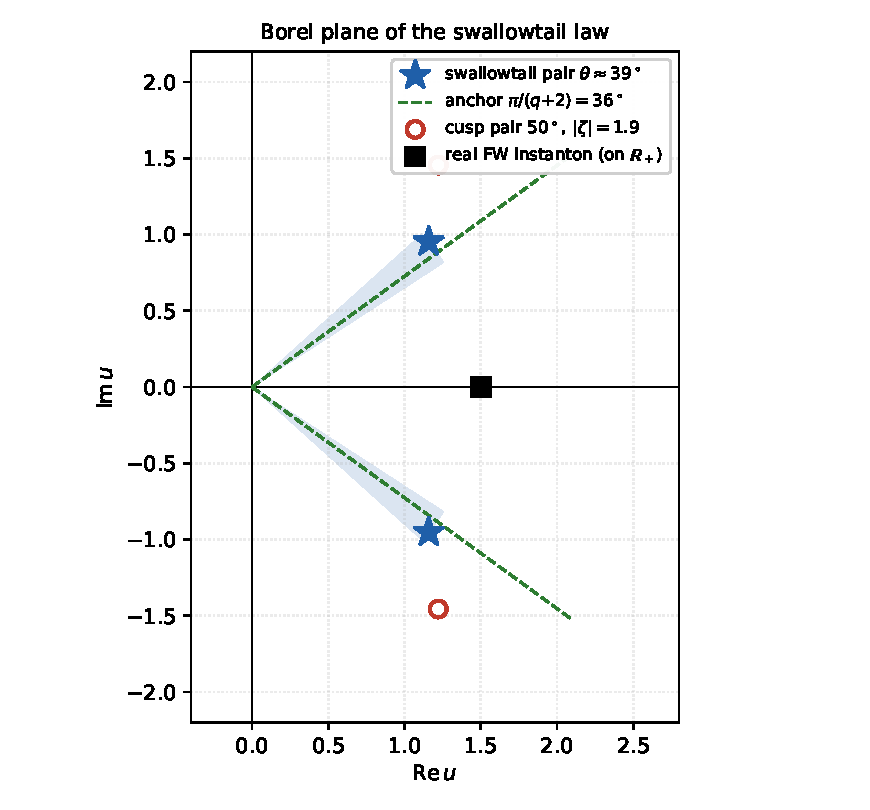
\includegraphics[width=0.58\textwidth]{swtl_fig_borel.pdf}
\caption{The Borel plane of $\Sw$. The conjugate pair (stars) sits at $|\zeta|\approx1.5$ with the
shaded wedge showing the method spread $\theta\in[33^\circ,42^\circ]$ of \eqref{eq:theta}; the
deterministic anchor $\pi/(q{+}2)=36^\circ$ \eqref{eq:anchorphase} is the dashed green ray, and lies
inside the wedge. The real Freidlin--Wentzell instanton \eqref{eq:instanton} (square) sits on
$\mathbb R_+$ at comparable modulus, so all three singularities compete --- which is why the
conjugate-pair conformal map fails (Section~\ref{sec:ledger}). The cusp pair (open circles,
$50^\circ$, $|\zeta|=1.9$) is shown for contrast: the swallowtail phase is smaller.}
\label{fig:borel}
\end{figure}

\begin{remark}[Status of \eqref{eq:anchorphase}]\label{rem:anchorstatus}
This is a pattern fixed by a single exactly-known case ($q=2$) and consistent with one measurement
($q=3$); it is not derived. What is imported is $\varphi=4\pi/(q+2)$ \cite{Voros1999}; the
identification of the root phase with $\varphi/4$ is ours and is conjectural.
\end{remark}

\section{Validation: what the trans-series reconstructs}\label{sec:resum}

Ground truth is Monte-Carlo free, from the escape Fokker--Planck PDE with a second-order
(MUSCL/van Leer) advection scheme. Two absolute gates fix its accuracy: at $x=0.09$ the
non-perturbative scale is $e^{-A\cos\theta/x}\sim e^{-13}$, so the converged partial sum \emph{is}
the exact answer, giving $+0.11\%$ ($q=2$) and $+0.35\%$ ($q=3$).

We resum by median/lateral Borel--Pad\'e: $B(u)=\sum_k(v_k/k!)u^k$, diagonal approximant, and
$f(x)=\int_0^\infty e^{-t}B(xt)\dd t$ on a contour rotated to $\pm\varphi$, the median
$\tfrac12(f_++f_-)$ being the physical value.

\begin{center}
\begin{tabular}{rrrrrrr}
\hline\noalign{\smallskip}
$x$ & $\beta$ & $f_{\rm exact}$ & 7-coef & err & 8-coef & err\\
\noalign{\smallskip}\hline\noalign{\smallskip}
0.09 & 44.4 & 0.056595 & 0.0564 & $-0.3\%$ & 0.0564 & $-0.3\%$\\
0.25 & 16.0 & 0.074659 & 0.0740 & $-0.8\%$ & 0.0735 & $-1.5\%$\\
0.49 &  8.2 & 0.104324 & 0.0859 & $-17.7\%$ & 0.1039 & $\mathbf{-0.4\%}$\\
0.81 &  4.9 & 0.133752 & 0.0753 & $-43.7\%$ & 0.1392 & $+4.1\%$\\
1.00 &  4.0 & 0.145188 & 0.0666 & $-54.1\%$ & \textbf{0.1563} & $\mathbf{+7.7\%}$\\
1.44 &  2.8 & 0.159783 & 0.0497 & $-68.9\%$ & 0.1877 & $+17.5\%$\\
2.00 &  2.0 & 0.164683 & 0.0354 & $-78.5\%$ & 0.2177 & $+32.2\%$\\
2.50 &  1.6 & 0.162948 & 0.0271 & $-83.4\%$ & 0.2396 & $+47.1\%$\\
\noalign{\smallskip}\hline
\end{tabular}
\end{center}

\begin{figure}[h]
\centering
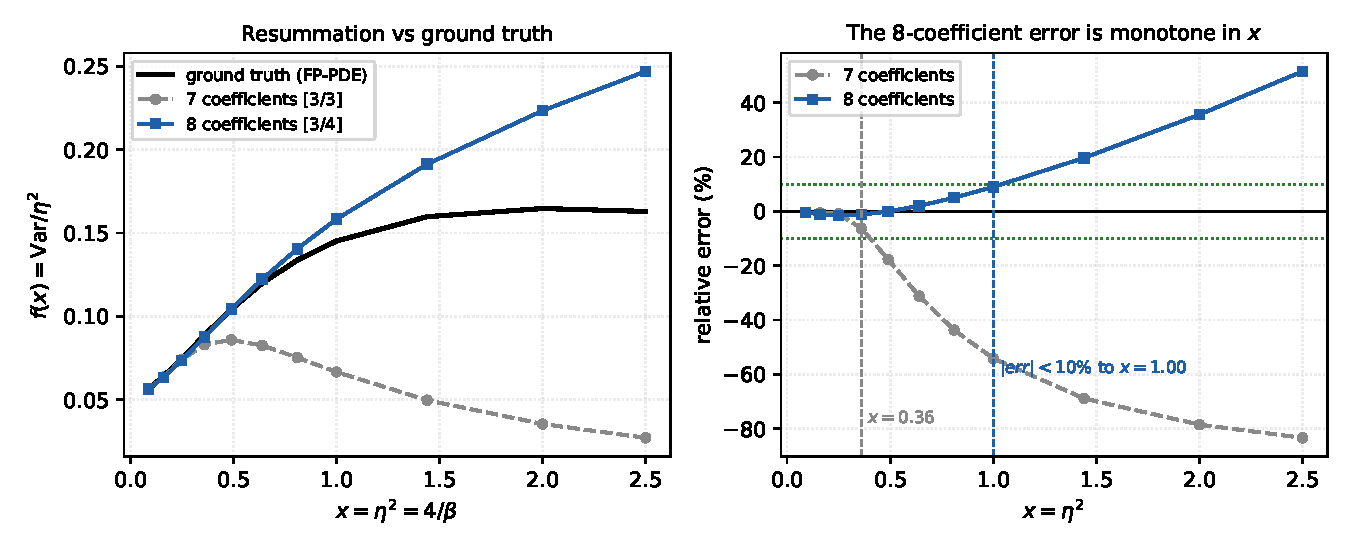
\includegraphics[width=0.95\textwidth]{swtl_fig_resum.pdf}
\caption{\emph{Left:} the resummed trans-series against Monte-Carlo-free ground truth. Seven
coefficients (grey) turn over and fall away; eight (blue) track the truth and, crucially, rise with
$x$ as they must. \emph{Right:} relative error. The eight-coefficient error is \emph{monotone}
in $x$ --- a radius-of-validity statement, not an unreliable approximant (Claim~\ref{claim:resum}).
The $|{\rm err}|<10\%$ range extends from $x\le0.36$ (seven coefficients) to $x\le1.00$, i.e.\
$\beta\ge4$, with eight.}
\label{fig:resum}
\end{figure}

\begin{claim}[The representation is sound; the approximant is starved]\label{claim:resum}
The eight-coefficient error is \emph{monotone} in $x$, never erratic in sign or size. This is a
radius-of-validity statement, not an unreliable approximant: the trans-series representation is
correct and the Pad\'e is simply starved outside its disc. The eighth coefficient roughly
\emph{triples} the reliable range --- $|{\rm err}|<10\%$ for $x\le1.00$ ($\beta\ge4$), against
$x\le0.36$ ($\beta\ge11$) with seven --- and reconstructs $\Var$ to better than $1\%$ for
$\beta\ge8$. Adding $v_7$ also flips the $\beta=2$ error from $79\%$ low to $32\%$ high, so the truth
is now bracketed. \tagN
\end{claim}

The $\beta=2$ ground truth is $\Var=0.3294$, with fingerprint skewness $+0.945$ and excess kurtosis
$+0.150$. Note the sign of the latter: the cusp's excess kurtosis at $\beta=2$ is \emph{negative}
($-0.243$). The steeper catastrophe is both more skewed and heavier-tailed; the cusp's sub-Gaussian
bulk signature does not carry over. \tagN

\section{Honest ledger}\label{sec:ledger}

\emph{Solid/exact:} the Bessel-$1/5$ skeleton and its zeros (Prop.~\ref{prop:bessel}); the
$\mathbb Z_5$ Stokes structure (Prop.~\ref{prop:z5}); the three obstructions
(Props.~\ref{prop:nofredholm}--\ref{prop:connection}); the exact one-loop coefficient
\eqref{eq:v0}; the instanton exponent $2q+1$.

\emph{Numerical but firm:} the eight-coefficient ladder \eqref{eq:coeffs} and its normalisation
check; the $\kappa_3$ ladder \eqref{eq:tcoeffs}; the same-rung sign flip across observables
(Claim~\ref{claim:sharedenvelope}); the instanton constant across $q=1,\dots,5$; the
reconstruction table of Section~\ref{sec:resum}; the ground truth $\Var(\beta{=}2)=0.3294$.

\emph{Numerical and soft:} the absolute value of $\theta$. Three estimators disagree by up to
$9^\circ$ and are reconciled only by cusp calibration; \eqref{eq:theta} should be read as
$33$--$42^\circ$, with the \emph{differential} statement ($8$--$17^\circ$ below the cusp) carrying
the weight. The top rung $v_7$ rests on a single usable grid point and has no band.

\emph{Open.} (i) $\beta=2$ is not reconstructed ($32\%$). (ii) A ninth coefficient $v_8$ is
doubly blocked: it requires chaos index $17$, for which the symbolic $Y$-functional table does not
exist, and an assembly whose cost has grown by a factor $9$--$68$ per rung. (iii) Two natural
methods for extracting the Borel data without more rungs were tried and \emph{refuted}, both
failing their cusp gate: a conformal map of the Borel plane (the pair map leaves the real instanton
strictly inside the unit disc, $|w|=0.01$--$0.22$), and direct extraction of the non-perturbative
remainder from the observable (the residual shows no oscillation and is method error, not the pair
term). Both fail for the same circular reason --- each needs $(A,\theta)$ as input. (iv) No
stochastic exact-WKB, as for the cusp.

\emph{The anchor was imported, and it does not rescue the resummation.} Since both refuted methods
needed $(A,\theta)$ as external input, we imported it (Rem.~\ref{rem:anchorexists}) and retried, in
two forms: a prescribed-singularity Borel ansatz
$B(u)=A_r(1-u/z_r)^{-g}+2\,\mathrm{Re}[A_p(1-u/\zeta)^{-g}]+\text{poly}$ with the pair angle fixed at
$\theta=\pi/(q+2)$ and the rest fitted; and a fully constrained version with $\theta,|\zeta|,z_r,g$
all fixed and only the (linear) amplitudes fitted. \emph{Both fail the cusp gate.} The fitted version
overfits catastrophically --- the residual goes to zero while $|\zeta|$ runs to $14$ and $f(2)$ to
$+1090\%$ --- because $8$ coefficients cannot support $9$--$11$ parameters. The constrained version
is far better behaved but still gives $+5\%$ at best on the cusp, against plain diagonal
Borel--Pad\'e's $-1.0\%$, and swings over $[-55\%,+43\%]$ across equally defensible choices of
$(|\zeta|,z_r,g)$.

\begin{remark}[Why structural priors do not substitute for coefficients]\label{rem:whypriorsfail}
The sensitivity just quoted is the explanation for all three refuted methods. At $x=2$ the resummed
value is exquisitely sensitive to Borel data we know only to $\sim20\%$ ($|\zeta|$) or hardly at all
($z_r$), so importing an exact $\theta$ does not help: the error budget is dominated by the
\emph{other} singularity data. Plain diagonal Pad\'e is hard to beat here precisely because it has
exactly as many parameters as coefficients and imports nothing. The binding constraint is therefore
the coefficient count itself, and structural priors enter with uncertainties that the sensitivity
amplifies rather than suppresses. Beating Pad\'e at $\beta=2$ would require $|\zeta|$ and $z_r$ to a
precision comparable to $\theta$'s --- i.e.\ a full TBA solution of the cubic Stokes data, not just
its phase. \tagN
\end{remark}

\begin{remark}[What the swallowtail adds to the cusp programme]
Three things. First, a structural one: solvability degrades with $q$
(Rem.~\ref{rem:lessintegrable}), so the multicritical family is not a uniform sequence of
equally tractable problems. Second, a quantitative one: the Borel phase is \emph{not} inherited
(Claim~\ref{claim:theta}), which any future inheritance theorem must accommodate. Third, a
methodological one: the same-rung sign flip across two independent observables
(Claim~\ref{claim:sharedenvelope}) is a Pad\'e-free diagnostic of Borel geometry, and the
$\kappa_3$ ladder --- an order of magnitude cheaper than the variance ladder --- is where that
diagnostic is cheapest to obtain.
\end{remark}

\section*{Acknowledgements}
Computations use the $q$-parameterised Wiener-chaos engine and the Fokker--Planck ground-truth
solver of the cusp programme, extended as described in the companion technical notes.

\begin{thebibliography}{99}

\bibitem{AllegrettiBridgeland} D.~Allegretti, T.~Bridgeland, \emph{The monodromy of meromorphic
projective structures}, arXiv:2006.10648. (Cubic-oscillator Stokes multipliers as cross-ratios and
Fock--Goncharov/Voros cluster coordinates, $\mathbb Z/5\mathbb Z$ pentagon structure; all-order WKB
expansion of the cluster coordinates with elliptic-period exponential scales.)

\bibitem{Voros1999} A.~Voros, \emph{Exact quantization condition for anharmonic oscillators (in one
dimension)}, arXiv:math-ph/9811001. (Complete constant set for the cubic: $\mu=5/6$,
$\varphi=4\pi/5$, $L=5$, $\kappa=1/5$, $b_0=2^{2/3}\sqrt3\,\Gamma(1/3)^3/(5\pi)$; exact quantisation
reproducing the spectrum to $10^{-6}$--$10^{-7}$.)

\bibitem{DoreyDunningTateo} P.~Dorey, C.~Dunning, R.~Tateo, \emph{The ODE/IM correspondence},
J.~Phys.~A \textbf{40} (2007) R205, arXiv:hep-th/0703066. (Stokes multiplier as an entire spectral
determinant of a lateral problem, fixed by $T$--$Q$/Bethe-ansatz or TBA/NLIE.)

\bibitem{Masoero2010} D.~Masoero, \emph{Y-system and deformed thermodynamic Bethe ansatz},
Lett.~Math.~Phys.~\textbf{94} (2010) 151--164.

\bibitem{ItoMarinoShu} K.~Ito, M.~Mari\~no, H.~Shu, \emph{TBA equations and resurgent quantum
mechanics}, JHEP \textbf{01} (2019) 228, arXiv:1811.04812.

\bibitem{Sibuya} Y.~Sibuya, \emph{Global Theory of a Second Order Linear Ordinary Differential
Equation with a Polynomial Coefficient}, North-Holland, 1975.

\bibitem{ClaeysKuijlaarsVanlessen} T.~Claeys, A.~B.~J.~Kuijlaars, M.~Vanlessen, \emph{Multi-critical
unitary random matrix ensembles and the general Painlev\'e II equation}, Ann.\ of Math.\
\textbf{168} (2008) 601--641.

\bibitem{BertolaCafasso} M.~Bertola, M.~Cafasso, \emph{Fredholm determinants and pole-free solutions
to the noncommutative Painlev\'e II hierarchy}, Comm.\ Math.\ Phys.\ \textbf{309} (2012) 793--833;
see also \emph{Higher order analogues of the Tracy--Widom distribution and the Painlev\'e II
hierarchy}, arXiv:0901.2473.

\bibitem{CafassoClaeys} \emph{Higher order analogues of Tracy--Widom distributions via the Lax
method}, arXiv:1208.3645.

\bibitem{MulticriticalSchur} \emph{Multicritical Schur measures and higher-order analogues of the
Tracy--Widom distribution}, arXiv:2307.05303.

\bibitem{AnicetoBaseSchiappa} I.~Aniceto, G.~Ba\c sar, R.~Schiappa, \emph{A primer on resurgent
transseries and their asymptotics}, Phys.\ Rep.\ \textbf{809} (2019) 1--135.

\bibitem{GaugeResurgence} \emph{Resurgent analysis of localizable observables in supersymmetric
gauge theories}, arXiv:1410.5834. (Different observables of one theory, shared and unshared Borel
singularity structure.)

\bibitem{BenderWu} C.~M.~Bender, T.~T.~Wu, \emph{Anharmonic oscillator}, Phys.~Rev.~\textbf{184}
(1969) 1231.

\bibitem{Dingle} R.~B.~Dingle, \emph{Asymptotic Expansions: Their Derivation and Interpretation},
Academic Press, 1973. (Late-terms/Darboux analysis used in \S\ref{sec:borel}.)

\bibitem{FW} M.~I.~Freidlin, A.~D.~Wentzell, \emph{Random Perturbations of Dynamical Systems},
3rd ed., Springer, 2012.

\bibitem{vanLeer} B.~van Leer, \emph{Towards the ultimate conservative difference scheme.~V},
J.~Comput.~Phys.~\textbf{32} (1979) 101--136. (MUSCL/limiter scheme used for the ground-truth
solver in \S\ref{sec:resum}.)

\end{thebibliography}

\end{document}
